% For directory trees
\usepackage{dirtree}

\subsection{Drasil}

\begin{frame}
    \frametitle{Drasil}
    \framesubtitle{What is Drasil?}
    My project was originally focused on Drasil, ``a framework for generating
    all of the software artifacts from a stable knowledge base, focusing
    currently on scientific software'' \citep{HuntEtAl2021}
    \vspace{-2mm}
    \begin{columns}[T,onlytextwidth]
        \begin{column}{.6\textwidth}
            \vspace{2mm}
            \begin{minipage}{\textwidth}
                \begin{itemize}
                    \item<2-> I worked on Drasil as an Undergraduate Summer
                          Research Assistant during the summers of 2018 and 2019
                          % \item<2-> Knowledge is introduced either at a global level
                          %     or at an example-specific level
                    \item<3-> ``Recipes'' specify how information from the
                          knowledge based is used to generate
                          software artifacts, including:
                          \begin{itemize}
                              \item SRS (HTML, PDF, Markdown)
                              \item Code (Python, Java, C\#, C++, Swift, Julia)
                              \item READMEs and Makefiles
                              \item Drasil's own website\footnotemark[1]!
                          \end{itemize}
                \end{itemize}
            \end{minipage}
        \end{column}
        \begin{column}{.35\textwidth}
            % \vspace{-4mm}
            \begin{figure}
                
\includegraphics[width=.8\textwidth]{assets/images/drasil_logo.png}
                \vspace{-2mm}
                \caption{Drasil's Logo \tiny\citep{Drasil}}
                \label{fig:drasil-logo}
            \end{figure}
        \end{column}
    \end{columns}
    \footnotetext[1]{\tiny \url{https://jacquescarette.github.io/Drasil/}}
\end{frame}

\begin{frame}
    \frametitle{Visualizing Drasil's Traceability}
    \begin{figure}
        \center
        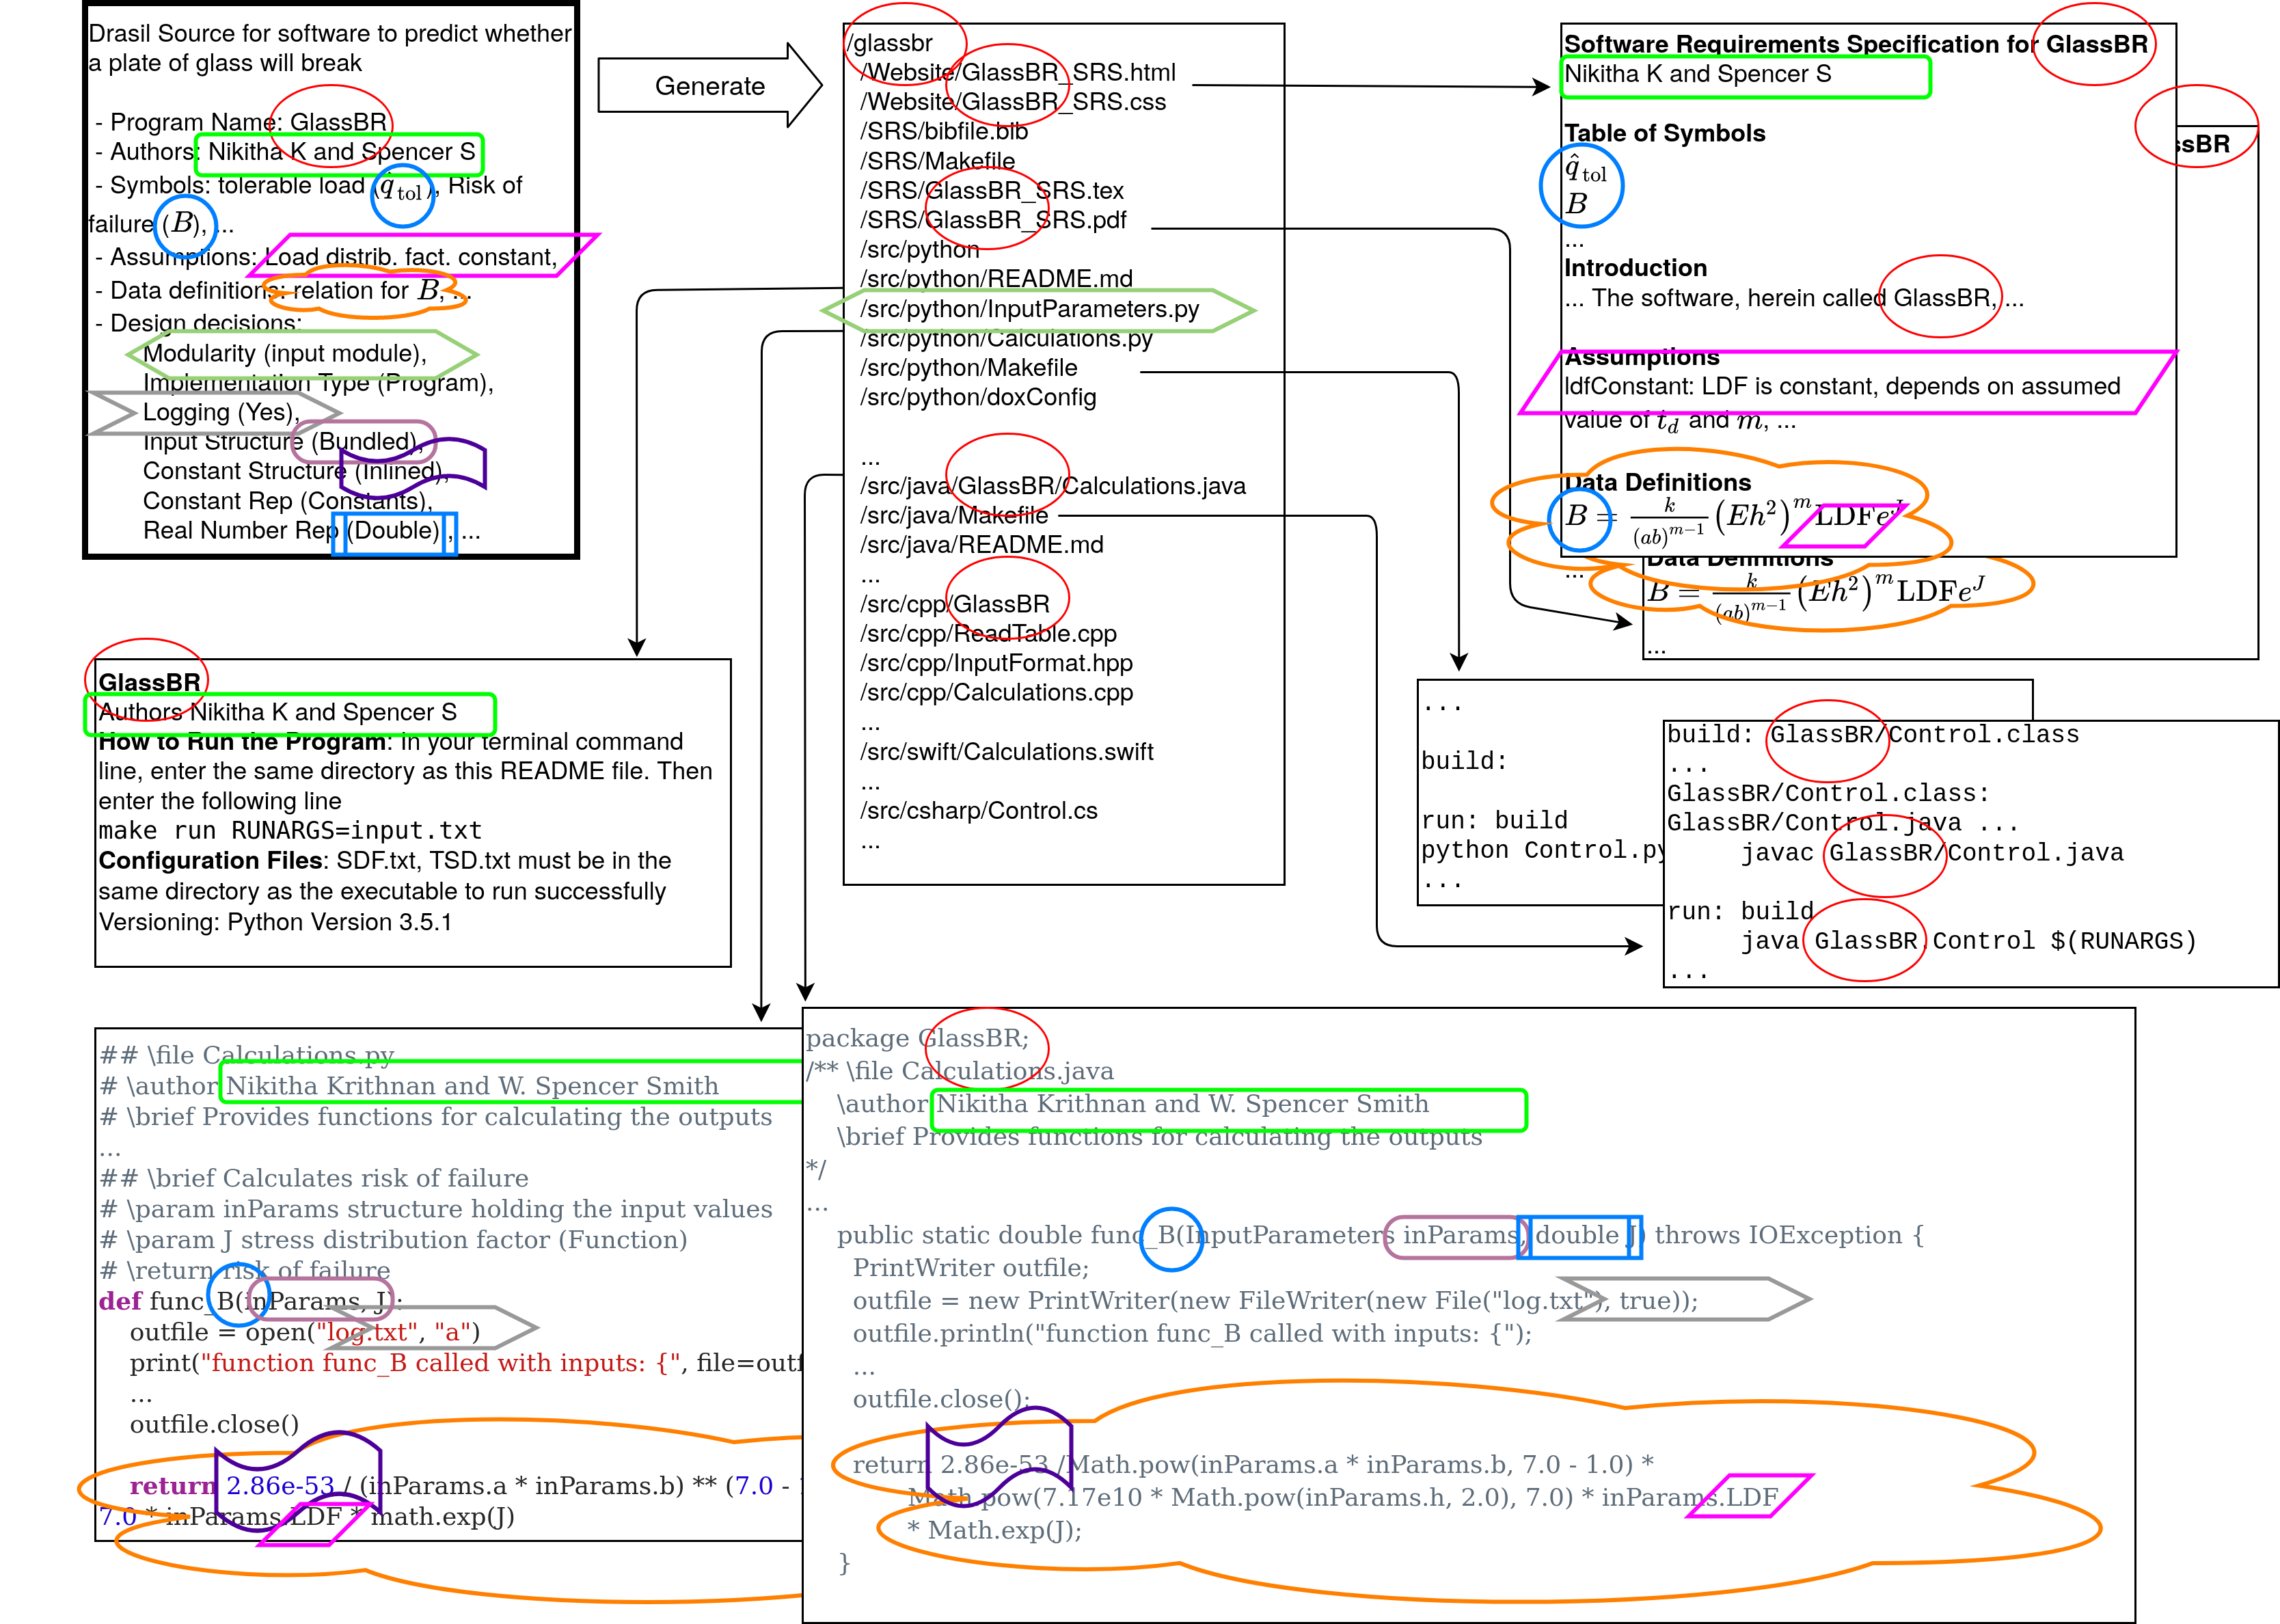
\includegraphics[width=0.8\textwidth]{assets/images/drasil_trace}
        \vspace{-2mm}
        \caption{Knowledge flow from knowledge base to artifacts; by Dr.~Spencer Smith}
        \label{fig:knowledge-flow}
    \end{figure}
\end{frame}

\begin{frame}
    \frametitle{Generating Test Cases}
    \framesubtitle{RIP to GOOT and TestGen}
    \begin{itemize}
        \item My project was originally going to be implementing
              test case generation in Drasil
        \item<2-> The rough workflow:
              \begin{enumerate}
                  \item<2-> Implement manual testing \\
                        Manual unit tests (26 \textcolor{green}{passed},
                        18 \textcolor{orange}{failed with known reason}) \\
                        Manual system tests (3 \textcolor{green}{passed},
                        4 \textcolor{orange}{failed with known reason})
                  \item<3-> Understand the {\only<5->{\color{red}}stable
                                knowledge base} to create new ``recipes''
                  \item<4-> Generate test cases!
              \end{enumerate}
        \item<5-> There was a big assumption in this plan that drastically
              changed my project
    \end{itemize}
\end{frame}

\begin{frame}
    \frametitle{The Need for a Knowledge Base}
    \begin{itemize}
        \item Drasil is built for ``(well understood) research software'' \citep{Drasil}
              based on knowledge of:
              \begin{enumerate}
                  \item<2-> Concepts used by the software,
                  \item<3-> Math used by the software or its derivation, and
                  \item<4-> Information used by Drasil used for generating artifacts
              \end{enumerate}
    \end{itemize}
    \renewcommand*\DTstyle{\ttfamily\tiny}
    \setlength{\DTbaselineskip}{5pt}
    \begin{columns}[T,onlytextwidth]
        \begin{column}<2->{.32\textwidth}
            \dirtree{%
                .1 (drasil-data package\footnotemark[2] part \#1).
                .2 Concepts.
                .3 Thermodynamics.hs.
                .3 Computation.hs.
                .3 Math.hs.
                .3 PhysicalProperties.hs.
                .3 Physics.hs.
                .3 SolidMechanics.hs.
                .2 Constraints.hs.
            }
        \end{column}
        \begin{column}<3->{.32\textwidth}
            \dirtree{%
                .1 (drasil-data package\footnotemark[2] part \#2).
                .2 Equations/Defining.
                .3 Derivations.hs.
                .3 Physics.hs.
                .2 Theories.
                .3 Physics.hs.
                .2 Units.
                .3 PhysicalProperties.hs.
                .3 Physics.hs.
                .3 SolidMechanics.hs.
                .3 Thermodynamics.hs.
                .2 SI\_Units.hs.
            }
        \end{column}
        \begin{column}<4->{.32\textwidth}
            \dirtree{%
                .1 (drasil-data package\footnotemark[2] part \#3).
                .2 Concepts.
                .3 Documentation.hs.
                .3 Education.hs.
                .3 Software.hs.
                .2 Software.
                .3 Products.hs.
                .2 Citations.hs.
                .2 People.hs.
            }
        \end{column}
    \end{columns}
    \only<2->{\footnotetext[2]{\tiny READMEs excluded for brevity; see \url{https://github.com/JacquesCarette/Drasil/tree/main/code/drasil-data/lib/Data/Drasil}}}
\end{frame}

\subsection{The Common Drasil Workflow}
\subsubsection*{Example: Projectile}

\begin{frame}
    \frametitle{The Common Drasil Workflow}
    \framesubtitle{Example: Projectile}

    \begin{columns}[T,onlytextwidth]
        \begin{column}{.25\textwidth}
            \begin{enumerate}
                \item<2-|handout:1-> Create a manual version of an artifact
                \item<3-|handout:2-> Understand it (and its components) well
                \item<4-|handout:3> Generate it!
            \end{enumerate}
        \end{column}
        \begin{column}{.75\textwidth}
            % \begin{overprint}
            %     \centering
            %     \onslide<2|handout:1>\begin{figure}
            %         \centering\includegraphics[width=.8\textwidth]{assets/projectile-sketch.PNG}
            %         \caption{Sketch of Projectile SRS \tiny \cite{projectile_sketch}}
            %     \end{figure}
            %     \onslide<3|handout:2>\begin{figure}
            %         \centering\includegraphics[width=.9\textwidth]{assets/projectile-wip.PNG}
            %         \caption{Review of Manual Projectile SRS \tiny \cite{projectile_wip}}
            %     \end{figure}
            %     \onslide<4|handout:3>\begin{figure}
            %         \centering\includegraphics[width=0.95\textwidth]{assets/projectile-current.PNG}
            %         \caption{HTML Version of Generated Projectile SRS \tiny \cite{projectile_current}}
            %     \end{figure}
            % \end{overprint}
        \end{column}
    \end{columns}

    % \begin{itemize}
    %     \item<2-> Create a manual version of an artifact
    %     \item<3-> Understand it (and its components) well
    %     \item<4-> Generate it!
    % \end{itemize}
    % \begin{columns}[T,onlytextwidth]
    %     \begin{column}{.3\textwidth}<3->
    %         \begin{figure}
    %             %   \vspace{-1mm}
    %             \includegraphics[width=.8\textwidth]{assets/projectile-sketch.PNG}
    %             %   \vspace{-3mm}
    %             \caption{Sketch of Projectile SRS}
    %             % \vspace{-1mm}
    %         \end{figure}
    %     \end{column}
    %     \begin{column}{.3\textwidth}<3->
    %         \begin{figure}
    %             %   \vspace{-1mm}
    %             \includegraphics[width=.8\textwidth]{assets/projectile-wip.PNG}
    %             %   \vspace{-3mm}
    %             \caption{Review of Manual Projectile SRS}
    %             % \vspace{-1mm}
    %         \end{figure}
    %     \end{column}
    %     \begin{column}{.3\textwidth}<3->
    %         \begin{figure}
    %             %   \vspace{-1mm}
    %             \includegraphics[width=.8\textwidth]{assets/projectile-current.PNG}
    %             %   \vspace{-3mm}
    %             \caption{HTML Version of Generated Projectile SRS\footnotemark[1]}
    %             % \vspace{-1mm}
    %         \end{figure}
    %     \end{column}
    % \end{columns}

    % \only<2->{\footnotetext[1]{\tiny \url{https://github.com/JacquesCarette/Drasil/blob/master/notes/ProjectileMotionSketchOfSRS.pdf}}}
    % \only<3->{\footnotetext[2]{\tiny \url{https://github.com/JacquesCarette/Drasil/blob/master/notes/FeedbackOnProjectile.tiff}}}
    % \only<4->{\footnotetext[3]{\tiny \url{https://jacquescarette.github.io/Drasil/examples/projectile/SRS/srs/Projectile_SRS.html\#Sec:Intro}}}
    % \vspace{-3mm}
\end{frame}

\subsubsection*{Applied to Testing}

\begin{frame}
    \frametitle{The Common Drasil Workflow}
    \framesubtitle{Applied to Testing}

    1. Create a manual version of an artifact
    \begin{itemize}
        % TODO: better colours
        \item Manual unit tests (26 \textcolor{green}{pass}, 18 \textcolor{orange}{fail with known reason})
        \item<5-|handout:4> Manual system tests (3 \textcolor{green}{pass}, 4 \textcolor{orange}{fail with known reason})
    \end{itemize}
    % \begin{overprint}
    %     \centering
    %     \onslide<2|handout:1>\begin{figure}
    %         \centering
    %         \lstinputlisting[
    %             title=Sample from \texttt{InputParameters\_test.py},
    %             captionpos=b,
    %             language=Python,
    %             basicstyle=\tiny, % TODO: make bigger
    %             firstline=17,
    %             lastline=23,
    %             breakatwhitespace=true,
    %             showstringspaces=false
    %         ]{assets/code/InputParameters_test.py}
    %     \end{figure}
    %     \onslide<3|handout:2>\begin{figure}
    %         \centering
    %         \lstinputlisting[
    %             title=Sample from \texttt{Calculations\_test.py},
    %             captionpos=b,
    %             language=Python,
    %             basicstyle=\tiny, % TODO: make bigger
    %             firstline=19,
    %             lastline=34,
    %             breakatwhitespace=true,
    %             showstringspaces=false
    %         ]{assets/code/Calculations_test.py}
    %     \end{figure}
    %     \onslide<4|handout:3>\begin{figure}
    %         \centering
    %         \lstinputlisting[
    %             title=Sample from \texttt{OutputFormat\_test.py},
    %             captionpos=b,
    %             language=Python,
    %             basicstyle=\tiny, % TODO: make bigger
    %             firstline=10,
    %             lastline=17,
    %             breakatwhitespace=true,
    %             showstringspaces=false
    %         ]{assets/code/OutputFormat_test.py}
    %     \end{figure}
    %     \onslide<6|handout:4>\begin{figure}
    %         \centering
    %         \lstinputlisting[
    %             title=Sample from \texttt{Control\_test.py},
    %             captionpos=b,
    %             language=Python,
    %             basicstyle=\tiny, % TODO: make bigger
    %             firstline=17,
    %             lastline=23,
    %             breakatwhitespace=true,
    %             showstringspaces=false
    %         ]{assets/code/Control_test.py}
    %     \end{figure}
    % \end{overprint}
\end{frame}

\begin{frame}
    \frametitle{The Common Drasil Workflow}
    \framesubtitle{Applied to Testing}

    2. Understand the manual artifact (and its components) well
    \begin{itemize}
        \item<2-> Changes made to "stable" to faciliate testing
              \begin{itemize}
                  \item The inclusion of \texttt{\_\_init\_\_.py} files to
                        improve \texttt{import} statements
                  \item Wrapping \texttt{Control.py}'s functionality in a
                        \texttt{main} function
                  \item Changing how command line parameters are
                        passed to \texttt{Control.py}
              \end{itemize}
        \item<3-> Changes to be made to generated code to improve correctness
              \begin{itemize}
                  \item Invalid values should stop the calculations
                        \cite{projectile_current}
                  \item Assumptions, such as values of constants, should be
                        verified
              \end{itemize}
    \end{itemize}
    % \vspace{2mm}
    % \begin{overprint}
    %     \centering
    %     \onslide<3>The inclusion of \texttt{\_\_init\_\_.py} files to
    %     improve \texttt{import} statements
    %     \onslide<4>Wrapping \texttt{Control.py}'s functionality in a
    %     \texttt{main} function
    %     \onslide<5>Changing how command line parameters are
    %     passed to \texttt{Control.py}
    %     \onslide<7>Invalid values should stop the calculations
    %     \cite{projectile_current}
    %     \onslide<8>Assumptions, such as values of constants, should be
    %     verified
    % \end{overprint}
    % \vspace{-4mm}
    % \begin{overprint}
    %     \centering
    %     \onslide<3>
    %     \begin{figure}
    %         \centering
    %         \lstinputlisting[
    %             title=Sample from \texttt{InputParameters\_test.py},
    %             captionpos=b,
    %             language=Python,
    %             basicstyle=\tiny, % TODO: make bigger
    %             firstline=12,
    %             lastline=15,
    %             breakatwhitespace=true,
    %             showstringspaces=false
    %         ]{assets/code/InputParameters_test.py}
    %     \end{figure}
    %     \vspace{-8mm}
    %     \begin{figure}
    %         \centering
    %         \lstinputlisting[
    %             title=Sample from \texttt{Control.py},
    %             captionpos=b,
    %             language=Python,
    %             basicstyle=\tiny, % TODO: make bigger
    %             firstline=7,
    %             lastline=9,
    %             breakatwhitespace=true,
    %             showstringspaces=false
    %         ]{assets/code/Control.py}
    %     \end{figure}
    %     \onslide<4>
    %     % TOOD: align better on page
    %     \begin{figure}[]
    %         % \centering
    %         \lstinputlisting[
    %             language=Python,
    %             basicstyle=\tiny, % TODO: make bigger
    %             firstline=11,
    %             lastline=11,
    %             breakatwhitespace=true,
    %             showstringspaces=false,
    %             % numbers=right % TODO: display line numbers for clarity
    %         ]{assets/code/Control.py}
    %     \end{figure}
    %     \vspace{-3mm}
    %     \begin{figure}
    %         % \centering
    %         \lstinputlisting[
    %             title=Sample of \texttt{Control.py},
    %             captionpos=b,
    %             language=Python,
    %             basicstyle=\tiny, % TODO: make bigger
    %             firstline=29,
    %             lastline=30,
    %             breakatwhitespace=true,
    %             showstringspaces=false,
    %             % numbers=right % TODO: display line numbers for clarity
    %         ]{assets/code/Control.py}
    %     \end{figure}
    %     \onslide<5>
    %     \begin{figure}
    %         \centering
    %         \lstinputlisting[
    %             title=Sample of \texttt{Control.py},
    %             captionpos=b,
    %             language=Python,
    %             basicstyle=\tiny, % TODO: make bigger
    %             firstline=13,
    %             lastline=16,
    %             breakatwhitespace=true,
    %             showstringspaces=false
    %         ]{assets/code/Control.py}
    %     \end{figure}
    %     \onslide<7>
    %     \begin{figure}
    %         \centering
    %         \lstinputlisting[
    %             language=Python,
    %             basicstyle=\tiny, % TODO: make bigger
    %             firstline=26,
    %             lastline=29,
    %             breakatwhitespace=true,
    %             showstringspaces=false,
    %             % numbers=right % TODO: display line numbers for clarity
    %         ]{assets/code/Control_test.py}
    %     \end{figure}
    %     \vspace{-8mm}
    %     \begin{figure}
    %         \centering
    %         \lstinputlisting[
    %             title=Sample of \texttt{Control\_test.py},
    %             captionpos=b,
    %             language=Python,
    %             basicstyle=\tiny, % TODO: make bigger
    %             firstline=37,
    %             lastline=43,
    %             breakatwhitespace=true,
    %             showstringspaces=false,
    %             % numbers=right % TODO: display line numbers for clarity
    %         ]{assets/code/Control_test.py}
    %     \end{figure}
    %     \onslide<8>
    %     \begin{figure}
    %         \centering
    %         \lstinputlisting[
    %             title=Sample from \texttt{Calculations\_test.py},
    %             captionpos=b,
    %             language=Python,
    %             basicstyle=\tiny, % TODO: make bigger
    %             firstline=52,
    %             lastline=68,
    %             breakatwhitespace=true,
    %             showstringspaces=false
    %         ]{assets/code/Calculations_test.py}
    %     \end{figure}
    % \end{overprint}
\end{frame}